%!TEX TS-program = xelatex 
%!TEX TS-options = -output-driver="xdvipdfmx -q -E"
%!TEX encoding = UTF-8 Unicode
%
%  summary_5
%
%  Created by Mark Eli Kalderon on 2009-03-04.
%

\documentclass[11pt]{article} 

% Definitions
\newcommand\myauthor{Mark Eli Kalderon} 
\newcommand\mytitle{Oxford Philosophy of Perception:}
\newcommand\mysubtitle{Prichard and the Sense Datum Fallacy}

% Packages
\usepackage{url}
\usepackage{txfonts}
\usepackage{color}
\definecolor{myblue}{rgb}{0.8,0.8,1}

% Define discussion environment
\makeatletter\newenvironment{discussion}{%
   \noindent\begin{lrbox}{\@tempboxa}\begin{minipage}{\columnwidth}\setlength{\parindent}{1em}}{\end{minipage}\end{lrbox}%
   \colorbox{myblue}{\usebox{\@tempboxa}}
}\makeatother

% XeTeX
\usepackage[cm-default]{fontspec}
\usepackage{xltxtra,xunicode}
\defaultfontfeatures{Scale=MatchLowercase,Mapping=tex-text}
\setmainfont{Hoefler Text}
\setsansfont{Gill Sans}
\setmonofont{Inconsolata}

% Title Information
\title{\mytitle\\
\mysubtitle}
\author{\myauthor} 
\date{} % Leave blank for no date, comment out for most recent date

% PDF Stuff
\usepackage[plainpages=false, pdfpagelabels, bookmarksnumbered, backref, pdftitle={\mytitle}, pagebackref, pdfauthor={\myauthor}, xetex, colorlinks=true, linkcolor=gray, urlcolor=gray]{hyperref}

%%% BEGIN DOCUMENT
\begin{document}

% Title Page
\maketitle

% Layout Settings
\setlength{\parindent}{1em}

% Main Content

\begin{figure}[htbp]
    \centering
        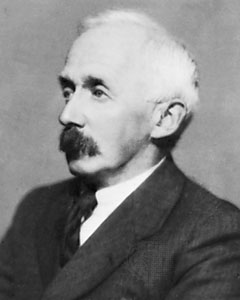
\includegraphics[scale=.5]{../../graphics/prichard.jpg}
    \caption{H.A. Prichard}
    \label{fig:prichard}
\end{figure}

\section{The Theory of Appearing} % (fold)
\label{sec:the_theory_of_appearing}
For Prichard, canonical appearance-attributions take the form:
    \begin{quote}
        \( o \) appears \( F \)
    \end{quote}
An \emph{appearance} is described by a canonical appearance-attribution. Prichard makes five central claims about appearances described by canonical appearance-attributions:
    \begin{enumerate}
        \item Appearance is presentational. An appearance is the \emph{appearing} of \( o \)---it is \( o \) appearing \( F \) to a subject \( S \).
        \item \( o \) is a body located in space.
        \item The predicate \( F \) has spatial conditions of application---it is intelligibly applied only to spatial bodies.
        \item The spatial body \( o \) is the object of the perception in virtue of which \( o \) appears.
        \item Our perception of \( o \) enables us to apprehend \( o \) and so come to know about it. In Prichard's later terminology, perception is a species of knowledge.
    \end{enumerate}

At least ever since ``Seeing Movement'' written in 1921, Prichard abandons the theory of appearing. Specifically, he denies that bodies are the object of perception, and he denies that perception is a species of knowledge.
% section the_theory_of_appearing (end)

\section{Perception as a Species of Knowledge} % (fold)
\label{sec:perception_as_a_species_of_knowledge}
While Prichard primarily casts his discussion in terms of \emph{knowledge}, various writers are held to be committed to the thesis that perception is a species of knowledge if in perceiving something the subject \emph{apprehends} it, is \emph{conscious} of it, or is \emph{aware} of it. There are important differences between these notions. Prichard is evidently thinking of knowledge as a genus of which these different attitudes are species.

\begin{discussion}
    Craig French wondered whether this really made sense. Normally, we think that perception affords awareness of things in our environment and this puts us in a position to know about these things. So understood, awareness is distinct from knowledge. Indeed, while knowledge takes a propositional object, awareness need not. 
    
    If Prichard's coherent, we must understand knowledge, as he understands it, in a more expansive sense. It is the most general category of certain kind of cognitive attitudes (cognitive in the sense that contrasts with conative and not in the sense that these attitudes are analyzable or otherwise reducible to beliefs.) This kind of cognitive attitude takes either propositional or nonpropositional objects. The relevant propositional attitudes are all \emph{factive}. The nonpropositional attitudes are all object involving in the sense that one can only have that attitude toward an object if that object exists.
\end{discussion}

The theory of appearing was a theoretical development of Cook Wilson's reflections on the nature of appearance. While Prichard abandons the theory of appearing, he retains, throughout his career, Cook Wilson's conception of knowledge. One feature of this conception is presently important:
\begin{quote}
    The object of knowledge is independent of the act of knowing.
\end{quote}
To maintain, then, that perception is a species of knowledge is to maintain that the object of perception is independent of the subject's perceiving it. Prichard's opposition to the idea that perception is a species of knowledge is motivated by the Berkelean contention that the objects of perception are dependent on perceiving them.

``The Sense Datum Fallacy'' falls into four parts:
\begin{enumerate}
    \item The first part introduces the theme of the paper. (1-3)
    \item The second part argues that a family of anti-idealist arguments belonging to a tradition inaugurated by Moore all turn on the thesis that perception is a species of knowledge. (4-7)>
    \item The third part argues against the thesis that perception is a species of knowledge. (7-12)
    \item The fourth part argues that the sense datum theory is committed to the problematic thesis that perception is a species of knowledge. (12-18)
\end{enumerate}
% section perception_as_a_species_of_knowledge (end)

\section{Introduction} % (fold)
\label{sec:introduction}
Prichard begins by considering two questions:
\begin{enumerate}
    \item What are the objects of peception?
    \item Do the objects of perception depend on the subject's perceiving them?
\end{enumerate}
And he contrasts the naïve realist's answer with Berkeley's.

According to the naïve realist:
\begin{enumerate}
    \item The objects of perception are bodies.
    \item Bodies are not dependent on our perceiving them.
\end{enumerate}
(Indeed, Prichard thinks that it is part of the meaning of ``body'' that a body is independent f our perception of it. So understood, ``external body'' is redundant.)

Berkeley in contrast maintains that:
\begin{enumerate}
    \item The objects of perception are secondary qualities. These have a ``common character''---they are sensations.
    \item Given the nature of sensations, they are dependent on a subject's perceiving them.
\end{enumerate}

Prichard observes that contemporary writers agree with Berkeley that the object's of perception are secondary qualities. But they maintain, instead, that these are sense data. And as a consequence, certain questions arise about the nature of sense data, that do not arise if secondary qualities are understood as sensations. Moreover, the substitution of sense data for sensations is fallacious in the sense that it depends on the false thesis that perception is a species of knowledge.

A couple of comments. First, this is not really a fallacy. Prichard is not charging the sense data theorist with \emph{invalid} reasoning so much as \emph{unsound} reasoning. Second, Prichard is emphasizing certain hard metaphysical questions about the nature of sense data that seem not to admit of determinate answers. In this way he is echoing G.A. Paul's worries about the persistence-conditions of sense data. However, whereas Paul maintains that these embarrassing questions only arise if the existence of sense data is regarded as a substantive metaphysical issue, Prichard seems not to consider the idea advocated by Paul and Ayer that the existence of sense data is not a substantive metaphysical issue.
% section introduction (end)

\section{The Anti-Idealist Arguments of Kemp Smith and Moore} % (fold)
\label{sec:the_anti_idealist_arguments_of_kemp_smith_and_moore}
Kemp Smith's argument:
\begin{enumerate}
    \item The objects of perception are secondary qualities.
    \item Secondary qualities are sensations.
    \item However, what Berkeley fails to notice is that sensation is ambiguous. A sensation may either be:
    \begin{enumerate}
        \item the object apprehended, or
        \item the act of apprehension
    \end{enumerate}
    \item The claim that secondary qualities are sensations is only true of sensations are understood as the objects of apprehension.
    \item Berkely thus fallaciously reasons from our perceiving sensations to tehese being dependent on our perceiving them. The subjective idealist claim only follows on the other reading of sensation. But so understood the claim is false.
    \item Further, if sensations are the objects of apprehension, then they are not dependent on our apprehension of them in perception.
\end{enumerate}

Both Moore's and Kemp Smith's arguments crucially depend on the thesis that perception is a species of knowledge. In Kemp Smith's argument, this is manifest in his claim that in seeing a color, the color is the object of apprehension.
% section the_anti_idealist_arguments_of_kemp_smith_and_moore (end)

\section{Why Perception is Not a Species of Knowledge} % (fold)
\label{sec:why_perception_is_not_a_species_of_knowledge}
Prichard gives three arguments:
\begin{enumerate}
    \item The supposition that the objects of perception existe independently of our perceiving them raises substantive metaphysical questions that admit of no determinate answers.
    \item The secondary qualities that we perceive depend on our perception of them and so perception is not a species of knowledge.
    \item If perceiving were a kind of knowing, mistakes would not be possible, but they are.
\end{enumerate}

First, suppose that Berkeley is right that the objects of perception are secondary qualities. But suppose that, contrary to Berkeley, perception is a species of knowledge. Then secondary qualities would exist independently of our perceiving them. But now, certain questions arise about the nature of these secondary qualities. Specifically questions about their publicity, persistence-conditions, their material or mental nature, and their causal origin. Kemp Smith accepts that these are substantive metaphysical questions but concedes that they admit of no determinate answers. Prichard insinuates, however, that if sense data really do exist, then there would be determinate answers to these questions.
    
\begin{discussion}
    Craig French wondered whether we should accept the claim that if sense data exist, then there are determinate answers to these metaphysical questions. There is no verificationist thought at work in the background as their might be with Ayer. I suspect that Prichard's argument here is meant to be nondemonstrative---the best explanation for why we lack determinate answers concerning the nature of sense data is that there are no such things.
\end{discussion}

Second, Berkeley and his modern opponents are right in thinking that what we perceive in each kind of perception is an appropriate kind of secondary quality. Berkeley however is right that the secondary qualities depend on our perception of them. Prichard supports this by asking us to consider the case of audition. Berkeley's claim that sounds are the primary objects of auditory experience is plausible. But even conceding this much to Berkeley seems not to obviously commit us to sounds being dependent upon our hearing them.

The third argument can \emph{seem} like a variant of the argument from illusion (though it really has a very different character):
\begin{quote}
    \ldots\ if perceiving were a kind of knowing, mistakes about what we perceive would be impossible, and yet they are constantly being made, since at any rate in the cases of seeing and feeling or touching we are almost always in a state of thinking that what we are perceiving are various bodies, although we need only to reflect to discover that in this we are mistaken.
\end{quote}

The passage is frustrating in its lack of explicitness. Indeed in the last line Prichard seems to echo Hume's contention that it takes the slightest bit of philosophy to show that naïve realism is false. Moreover you will struggle to find any explicit, worked out version of this argument in any of Prichard's work.

Although, we have, perhaps, seen a previous version of this argument put forward by an interlocutor in the chapter ``Phenomenalism and Things in Themselves'' of \emph{Kant's Theory of Knowledge}:
\begin{quote}
    \ldots\ if we maintain that we perceive the real lines, we may reasonably be asked whether we must not under all circumstances perceive them as they are. It seems as though a reality cannot be perceived except as it is. \emph{Kant's Theory of Knowledge}, 82
\end{quote}
If that is right, then Prichard has obviously grown dissatisfied with his earlier response that a spatial body appearing other than it is is made possible and necessary by the nature of space.

\begin{discussion}
    Paul Snowdon made the important suggestion that this argument turns on a special feature of the Cook Wilsonian conception of knowledge:
    \begin{quote}
        The consciousness that the knowing process is a knowing process must be contained within the knowing process itself. \emph{Statement and Inference}, 107
        
        [knowledge cannot be one of] two states of mind \ldots\ the correct and the erroneous one \ldots\ quite indistinguishable to the man himself. [For] as the man does not know in the erroneous state of mind, neither can he know in the other state. \emph{Statement and Inference}, 107
    \end{quote}
Prichard himself accepts this commitment:
\begin{quote}
    Consider instances: when knowing, for example, that a noise we are hearing is loud, we do or can know that we are knowing this and so cannot be mistaken, and when believing that the noise is due to a car we know or can know that we are believing and not knowing this. ``History of the Theory of Knowing'', \emph{Knowledge and Perception}, 89
\end{quote}

If perception were a species of knowledge, it would contain within itself the knowing process. Whatever that means more precisely, it at least entails that in perceiving something we know that we perceive it. Conversely, if we do not perceive something then we know that we do not. But now consider that we naturally take ourselves to perceive bodies. However, we do not perceive bodies---``we need only to reflect to discover that in this we are mistaken''. If perception were really, then, a species of knowledge we would know that we are not perceiving bodies. And, hence, perception is not a species of knowledge.

This may very well reveal a tension within the Oxford realism of Cook Wilson and Prichard. If Cook Wilson and early Prichard were right that realism requires that the objects of perception be independent of our perceiving them, then this can only be retained by abandoning a feature of the Cook Wilsonian conception of knowledge. It is perhaps telling then that Austin jettison's this feature of Cook Wilson's conception of knowledge.
\end{discussion}
% section why_perception_is_not_a_species_of_knowledge (end)

\section{Sense Datum and Perception as a Species of Knowledge} % (fold)
\label{sec:sense_datum_and_perception_as_a_species_of_knowledge}
Prichard's exposition proceeds by examining Russell's conception of sense datum. However, we need not follow him in this. Let experience be the genus of which perception is a species. The sense datum theorist maintains that there is something of which a subject is \emph{aware} in undergoing an experience. A sense datum, then, is just whatever plays this epistemic role. Given this characterization, it is \emph{further} argument that establishes substantive claims about the nature of sense data. This is roughly how Moore and Price understood matters. Notice, so introduced sense data do presuppose, in Prichard's vocabulary, that perceiving is a species of knowledge.

Prichard argues that so understood there is no such thing as sense data. By which he means that there is no \emph{kind} of thing which is a sense data. There is no ``common characteristic'' to sense data the way there is with Berkelean sensations. Here Prichard is anticipating a line of reasoning involved in Austin's complaint that material objects and sense data take in each other's washing. If the distinction between material objects and sense data is intelligible, then one of these categories must be united by a kind and the other must consist in all things that are not of that kind. Austin's argument now involves the conjunction of two claims: that there is no kind that unites material objects---they must be understood as non-sense-data; that there is no kind that unites sense data---they must be understood as non-material-objects. Prichard's argument here anticipates Austin's second claim. 
% section sense_datum_and_perception_as_a_species_of_knowledge (end)

\end{document}
